\chapter{Быстрые системы}

\section{Введение}

\noindent Рассмотрим следующую систему:

\begin{itemize}
	\item Конвейеры имеют всюду равномерную скорость $v$, притом достаточно большую, чтобы можно было пренебречь взаимодействием между ресурсами, и преодолеваемыми ими расстояниями (а соответственно -- и временем)
	
	\item Конвейерные разъединители работают по следующим правилам:
		\begin{itemize}
			\item Всевозможные их числа выходов образуют множество $\mathbb{T} = \{ t_1, ..., t_n \}$
			\item Правило вывода: чередовать ресурс между выходами 
				
				Схема очерёдности:
				
				\vspace{0.25in}
				
				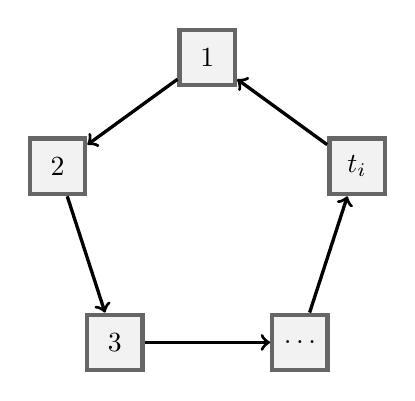
\begin{tikzpicture}[
					a/.style={rectangle, draw=black!60, fill=black!5, ultra thick, minimum size=20}
					]
					
					%Nodes
					\node[a] (1)   at (0, 2) 		   {$1$};
					\node[a] (2)   at (-1.902, 0.618)  {$2$};
					\node[a] (3)   at (-1.176, -1.618) {$3$};
					\node[a] (etc) at (1.176, -1.618)  {$\ldots$};
					\node[a] (i)   at (1.902, 0.618)   {$t_i$};
					
					%Lines
					\draw[->, very thick] (1) to (2);
					\draw[->, very thick] (2) to (3);
					\draw[->, very thick] (3) to (etc);
					\draw[->, very thick] (etc) to (i);
					\draw[->, very thick] (i) to (1);
				\end{tikzpicture}
				
			\item При этом распределение происходит мгновенно: как только ресурс заходит -- так только и выходит
				
		\end{itemize}
		
	\item Конвейерный соединитель может принимать любое число ресурсов, и мгновенно объединяет их в один конвейер (очерёдность не важна, т.к. ресурсы друг с другом не взаимодействуют)
	
\end{itemize}





\vspace{0.25in}

\noindent Всвязи с мгновенностью распределений, назовём такую систему "быстрой".

\vspace{0.4in}

\noindent В быстрых системах определён следующий набор действий:

\begin{itemize}
	\item Разделение (англ: splitting/chopping) -- разделение одного конвейера на $n$ равных частей
	
		%\begin{tikzpicture}[
		%	o/.style={rectangle, draw=green!60, fill=green!5, thick, minimum size=20},
		%	s/.style={rectangle, draw=blue!60,  fill=blue!5,  thick, minimum size=20},
		%	r/.style = {->, thick, rounded corners=10pt}
		%	]
		%	
		%	%Nodes
		%	\node[o]	(in)	at	(-2, 0)	{in};
		%	\draw[draw=blue!60,	fill=blue!5] (-0.5, 1) rectangle node {$s$} (0.5, -1);
		%	\node[o]	(out1)	at	(2, 2)	{$1$};
		%	\node[o]	(oute)	at	(2, 0)	{$\ldots$};
		%	\node[o]	(outn)	at	(2, -2)	{$n$};
		%	
		%	%Lines
		%	\draw[r]	(in.east)	to	node[above]			{$n$}	(-0.5, 0);
		%	\draw[r]	(0, 1) 		|-	node[below right]	{$1$}	(out1.west);
		%	\draw[r]	(0.5, 0) 	to	node[above]			{$1$}	(oute.west);
		%	\draw[r]	(0, -1) 	|-	node[above right]	{$1$}	(outn.west);
		%	
		%\end{tikzpicture}
		
	
	\item Соединение (англ: merging) -- соединение $n$ конвейеров в один
		
	\item Возврат (англ: re-looping/re-cycling) -- сначала отделение некоторой части потока, а затем соединение этой части с началом самого потока
	
		Пример:
		
		\begin{tikzpicture}[
			s/.style={rectangle, draw=black!60, fill=black!5, thin, minimum size=20},
			a/.style={rectangle, draw=black!60, fill=black!5, thin, minimum size=20},
			o/.style={rectangle, draw=black!60, fill=black!5, thin, minimum size=20},
			]
			
			%Nodes
			\node[a]    (a1)                          	{a};
			\node[s]    (s1)        [above = of a1]     {s};
			\node[s]    (s2)        [left = of s1]      {s};
			\node[o]	(in1)		[below = of a1]		{in};
			\node[a]    (a2)        [above = of s1]   	{a};
			\node[o]	(out1)		[above = of a2]		{out};
			\node[o]	(out2)		[left = of out1]	{out};
			
			%Lines
			\draw[->, thin] (in1.north) to node[right] 	 			  {$1$} 		  (a1.south);
			\draw[->, thin] (a1.north)  to node[right] 	 		 	  {$\frac{6}{5}$} (s1.south);
			\draw[->, thin] (s1.west)   to node[above] 	 		 	  {$\frac{2}{5}$} (s2.east);
			\draw[->, ultra thick] (s2) to[bend left=-45] node[left]  {$\frac{1}{5}$} (a1);
			\draw[->, thin] (s1.north)  to node[right] 				  {$\frac{2}{5}$} (a2.south);
			\draw[->, thin] (s1) 	    to[bend right=90] node[right] {$\frac{2}{5}$} (a2);
			\draw[->, thin] (a2.north)  to node[right] 	 			  {$\frac{4}{5}$} (out1.south);
			\draw[->, thin] (s2.north)  to node[left]	 			  {$\frac{1}{5}$} (out2.south);
		\end{tikzpicture}
		
	\item Отделение%
	\footnote{\textbf{Раз}деление и \textbf{от}деление отличаются тем, что \textbf{Раз}деление -- это построение n-арного дерева; а \textbf{от}деление -- это построение второй ветви, по которой едет заданное число ресурсов. Более заметно это различие в английской терминологии, а в русской различие заключается лишь приставкой...}
	(англ: separating) -- набор из последовательных и параллельных разделений, соединений и возвратов, с целью отделения заданой части $q_1$ ресурсов от изначальной конвейерной ленты, перевозящей $q_0$ ресурсов ($q_1 < q_0$)
		
		
\end{itemize}














\vspace{0.5in}


Назовём все числа вида $s = \prod_{i=1}^n t_i^{a_i}$ , где $a_i \in \mathbb{N}_0$ "стандартными". Тогда каждое число, \underline{обратное стандартному}%
\footnote{Будем называть такие числа единичными стандартными, или просто единичными. А если в числителе стоит не единица -- то будем называть их стандартными долями.} 
может быть получено, как отделение от конвейера в 1 при помощи смеси $t_1$-арного,~...~,~и $t_n$-арного деревьев.






\vspace{0.5in}

\section{Теорема о числе перестановок}

\

Для множества $\mathbb{T} = \{2, 3\}$ , число $2^13^1=6$ является стандартным, тогда $1/6$ является единичной дробью, её можно получить двумя способами:





\vspace{0.25in}

\begin{minipage}{0.4\textwidth}
	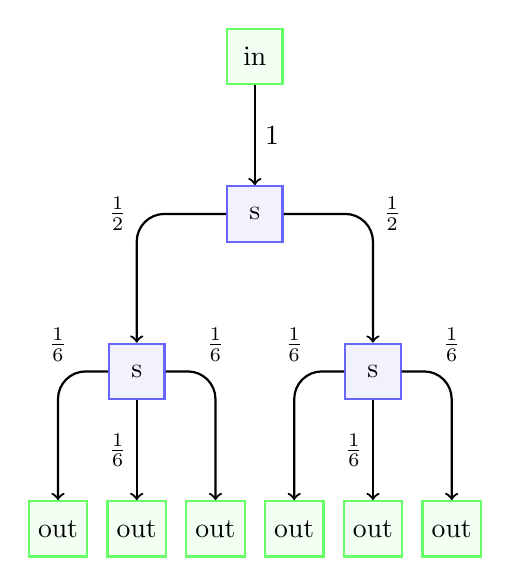
\begin{tikzpicture}[
		s/.style = {rectangle, draw=blue!60, fill=blue!5, thick, minimum size=20},
		a/.style = {rectangle, draw=red!60, fill=red!5, thick, minimum size=20},
		o/.style = {rectangle, draw=green!60, fill=green!5, thick, minimum size=20},
		r/.style = {->, thick, rounded corners=10pt}
		]
		
		%Nodes
		\node[o]	(in1)	at (0, 2)		{in};
		\node[s]	(s1)	at (0, 0)		{s};
		\node[s]	(s2)    at (-1.5, -2)	{s};
		\node[s]	(s3)    at (1.5, -2)	{s};
		\node[o]	(out1)	at (-2.5, -4)	{out};
		\node[o]	(out2)	at (-1.5, -4)	{out};
		\node[o]	(out3)	at (-0.5, -4)	{out};
		\node[o]	(out4)	at (0.5, -4)	{out};
		\node[o]	(out5)	at (1.5, -4)	{out};
		\node[o]	(out6)	at (2.5, -4)	{out};
		
		%Lines
		\draw[->, thick] (in1.south) to node[right] {$1$} 			(s1.north);
		\draw[->, thick] (s2.south)  to node[left]  {$\frac{1}{6}$} (out2.north);
		\draw[->, thick] (s3.south)  to node[left]  {$\frac{1}{6}$} (out5.north);
		
		\draw[r] (s1.west) -| node[left]   {$\frac{1}{2}$} (s2.north);
		\draw[r] (s1.east) -| node[right]  {$\frac{1}{2}$} (s3.north);
		\draw[r] (s2.west) -| node[above]  {$\frac{1}{6}$} (out1.north);
		\draw[r] (s2.east) -| node[above]  {$\frac{1}{6}$} (out3.north);
		\draw[r] (s3.west) -| node[above]  {$\frac{1}{6}$} (out4.north);
		\draw[r] (s3.east) -| node[above]  {$\frac{1}{6}$} (out6.north);
		
	\end{tikzpicture}
\end{minipage}
\hspace{50pt}
\begin{minipage}{0.4\textwidth}
	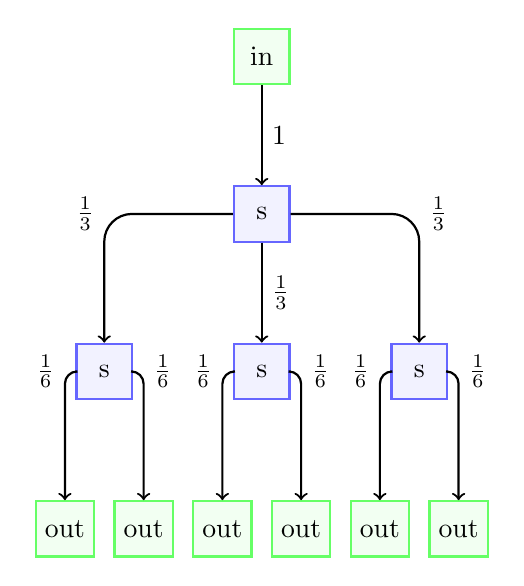
\begin{tikzpicture}[
		s/.style={rectangle, draw=blue!60, fill=blue!5, thick, minimum size=20},
		a/.style={rectangle, draw=red!60, fill=red!5, thick, minimum size=20},
		o/.style={rectangle, draw=green!60, fill=green!5, thick, minimum size=20},
		r1/.style = {->, thick, rounded corners=10pt},
		r/.style = {->, thick, rounded corners=4.5pt}
		]
		
		%Nodes
		\node[o]	(in1)	at (0, 2)		{in};
		\node[s]	(s1)	at (0, 0)		{s};
		\node[s]	(s2)	at (-2, -2)		{s};
		\node[s]	(s3)    at (0, -2)		{s};
		\node[s]	(s4)    at (2, -2)		{s};
		\node[o]	(out1)	at (-2.5, -4)	{out};
		\node[o]	(out2)	at (-1.5, -4)	{out};
		\node[o]	(out3)	at (-0.5, -4)	{out};
		\node[o]	(out4)	at (0.5, -4)	{out};
		\node[o]	(out5)	at (1.5, -4)	{out};
		\node[o]	(out6)	at (2.5, -4)	{out};
		
		%Lines
		\draw[->, thick] (in1.south) to node[right] {$1$} 			(s1.north);
		\draw[r1] 		 (s1.west) 	 -| node[left]  {$\frac{1}{3}$} (s2.north);
		\draw[->, thick] (s1.south)  to node[right] {$\frac{1}{3}$} (s3.north);
		\draw[r1] 		 (s1.east)   -| node[right] {$\frac{1}{3}$} (s4.north);
		
		\draw[r] (s2.west) -| node[left]  {$\frac{1}{6}$} (out1.north);
		\draw[r] (s2.east) -| node[right] {$\frac{1}{6}$} (out2.north);
		\draw[r] (s3.west) -| node[left]  {$\frac{1}{6}$} (out3.north);
		\draw[r] (s3.east) -| node[right] {$\frac{1}{6}$} (out4.north);
		\draw[r] (s4.west) -| node[left]  {$\frac{1}{6}$} (out5.north);
		\draw[r] (s4.east) -| node[right] {$\frac{1}{6}$} (out6.north);
		
	\end{tikzpicture}
\end{minipage}

\newpage

Как можем заметить, дробь одна, а варианта её воспроизводства -- два. Отсюда сформулируем теорему:

\

Любую единичную дробь, инициализированную числом  $s = \prod_{i=1}^n t_i^{a_i}$ можно построить числом способов, равным числу перестановок его сомножителей:

$$
	\text{P}\left[ \sum_{i=1}^{n} a_i \right] \left( a_1, a_2, \ldots, a_n \right) 
	=
	\dfrac{\left[ \sum\limits_{i=1}^{n} a_i \right]!}{\prod\limits_{i=1}^{n} \left( a_i! \right)}
$$











\vspace{0.5in}

\section{Теорема о делимости}

\

Если некоторую стандартную долю конвейера $\frac{a}{s} \ (a < s)$ возвратить в его начало -- то на участке до начала отделения пойдёт $q_0 + \frac{a}{s}\cdot q_0$ , после второй рекурсии -- $q_0 + \frac{a}{s}\cdot \left( q_0 + \frac{a}{s}\cdot q_0 \right)$ , и так далее.

\

\noindent Таким образом, в конечном итоге по данному участку будет идти:

$$\sum_{i=0}^{\infty} q_0 \cdot \left( \frac{a}{s} \right)^i = q_0 \cdot \frac{1}{1-\frac{a}{s}} = q_0\cdot\frac{s}{s-a}$$

\

Так как $a$ можно выбрать произвольное -- то от конвейера можно отделить даже не стандартную долю.

\vspace{0.3in}

\noindent Обозначим операцию преобразования дроби $\frac{a}{s}$ в дробь $\frac{a}{b} \ (b \le s)$ за:

\begin{align*}
	&\frac{a}{s} - \frac{s-b}{s} := \frac{a}{s} \cdot \frac{1}{1 - \frac{s-b}{s}} = \frac{a}{b} \\	
	&\frac{a}{s} - \frac{b}{s} := \frac{a}{s} \cdot \frac{1}{1 - \frac{b}{s}} = \frac{a}{s-b}
\end{align*}

\vspace{0.3in}

Теорема: любой единичный конвейер можно разделить на любые два положительных рациональных, в сумме дающих единицу, как рациональные доли входного конвейера при помощи операций отделения и возврата

\begin{align*}
	&\forall \ q_0, q_1, q_2 \in \mathbb{Q}^+_0 \ (q_1 + q_2 = q_0) \ : \\
	&\exists \ a, b, s \in \mathbb{N}_0 \ (a, b \le s) \ (s - \text{standart}) \ | \\
	&q_1 = \frac{a}{s} - \frac{b}{s} \ , \ q_2 = \frac{s-a-b}{s} - \frac{b}{s}
\end{align*}












\vspace{0.5in}

\section{Теорема об упрощении}

\

\noindent Назовём системы:

\begin{itemize}
	\item "простыми", если: $\forall \ t_i \in \mathbb{T} \ : \ t_i$ -- простое
		
		Пример: $\mathbb{T} = \{2, 3\}$, $\mathbb{T} = \{11, 23, 41\}$, $\mathbb{T} \subseteq \{2, 3, 5, 7, 11, 13, \ldots\}$
	
	\item "полупростыми", если: $\forall t_i, t_j \in \mathbb{T} \ : \ \gcd(t_i; \ t_j) = 1$
	
		Пример: $\mathbb{T} = \{2, 3\}$, $\mathbb{T} = \{4, 9\}$, $\mathbb{T} = \{6, 7, 25\}$
	
	\item "дублирующими", если: $\exists \ t, a, b \in \mathbb{T} \ ; \ x \in \mathbb{N}_0 \ ; \ y, z \in \mathbb{N} \ | \ t^z = a^x b^y$
	
		Пример: $\mathbb{T} = \{2, 3, 6\}$, $\mathbb{T} = \{2, 4\}$, $\mathbb{T} = \{4, 6, 9\}$
\end{itemize}

\

Теорема: любую дублирующую систему можно упростить:

\begin{align*}
	&\forall \ \mathbb{T} \ | \ \exists \ t, a, b \in \mathbb{T} \ ; \ x \in \mathbb{N}_0 \ ; \ y, z \in \mathbb{N} \ | \ t^z = a^x b^y \ : \\
	&\exists \ \mathbb{T}' = \mathbb{T} \setminus \{t \ : \ \exists \ t, a, b \in \mathbb{T} \ ; \ x \in \mathbb{N}_0 \ ; \ y, z \in \mathbb{N} \ | \ t^z = a^x b^y \} \ne \emptyset \\
	&\mathbb{T}' - \text{prime, or half-prime}
\end{align*}

\

Таким образом не имеет смысла отдельно изучать дублирующие системы, ведь для них будут верны все свойства полупростых (и простых соответственно). Однако сами по себе дублирующие сисемы могут быть удобны в решении отдельных задачь: например, если в $t = \prod_i t_i^{a_i}$, \\ $\sum_i a_i$ -- достаточно большое -- то:

\begin{enumerate}
	\item Система, реализующая единичную дробь, инициализированную данным числом, будет банально громоздкой
	\item Возможных способов реализации такой системы тоже будет много, что значительно усложняет решение задачи
\end{enumerate}

\noindent Тогда действительно проще установить готовый разветвитель, а не строить его с нуля.




\newpage

\section{Алгебра задачи}

\subsection{Теория групп}

\

Так же хочется отметить, что каждый разделитель образует циклическую группу $C_{t_i}$ -- тогда резонно сказать, что конвейер в начале своего пути является циклической группой $C_1$, а каждый раз, применяя к нему операцию разделения при помощи серии параллельных сплиттеров, мы, по сути, домножаем группу конвейера на группу сплиттера:






\vspace{0.5in}


\begin{minipage}{0.4\textwidth}
	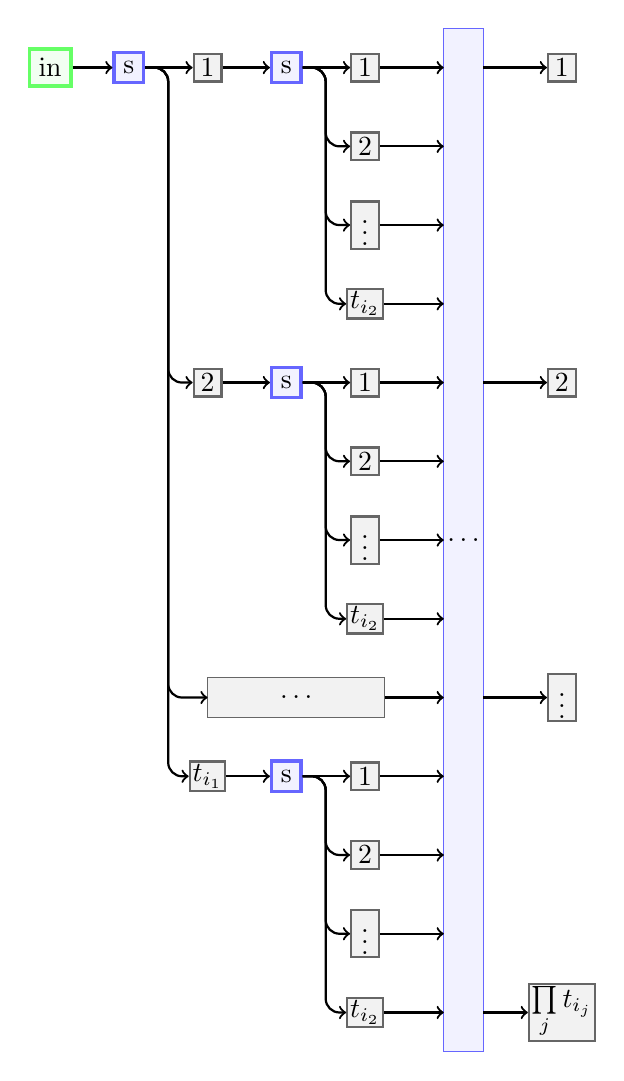
\begin{tikzpicture}[
		s/.style = {rectangle,	draw=blue!60,	fill=blue!5,	very thick, minimum size=10},
		a/.style = {rectangle,	draw=red!60,	fill=red!5,		very thick, minimum size=10},
		o/.style = {rectangle,	draw=green!60,	fill=green!5,	very thick, minimum size=10},
		t/.style = {rectangle,	draw=black!60,	fill=black!5,	thick, 		minimum size=10, inner sep=1pt},
		r/.style = {->, thick, rounded corners=5pt}
		]
		
		%Nodes
		\node[o]	(in)	at	(-3, 0)		{in};
		
		\node[s]	(s1)	at	(-2, 0)		{s};
		\node[t]	(t11)	at	(-1, 0)		{$1$};
		\node[t]	(t12)	at	(-1, -4)	{$2$};
		%\node[t]	(t1e)	at	(-1, -8)	{$\vdots$};
		\node[t]	(t1i)	at	(-1, -9)	{$t_{i_1}$};
		
		\node[s]	(s11)	at	(0, 0)		{s};
		\node[t]	(t121)	at	(1, 0)		{$1$};
		\node[t]	(t122)	at	(1, -1)		{$2$};
		\node[t]	(t12e)	at	(1, -2)		{$\vdots$};
		\node[t]	(t12i)	at	(1, -3)		{$t_{i_2}$};
		
		\node[s]	(s21)	at	(0, -4)		{s};
		\node[t]	(t221)	at	(1, -4)		{$1$};
		\node[t]	(t222)	at	(1, -5)		{$2$};
		\node[t]	(t22e)	at	(1, -6)		{$\vdots$};
		\node[t]	(t22i)	at	(1, -7)		{$t_{i_2}$};
		
		\node[s]	(si1)	at	(0, -9)		{s};
		\node[t]	(ti21)	at	(1, -9)		{$1$};
		\node[t]	(ti22)	at	(1, -10)	{$2$};
		\node[t]	(ti2e)	at	(1, -11)	{$\vdots$};
		\node[t]	(ti2i)	at	(1, -12)	{$t_{i_2}$};		
		
		% etc
		\draw[draw=blue!60,		fill=blue!5]	(2, 0.5)	rectangle node {$\ldots$} (2.5, -12.5);
		\draw[draw=black!60,	fill=black!5]	(-1, -7.75)	rectangle node {$\ldots$} (1.25, -8.25);
		
		\node[t]	(t1)	at	(3.5, 0)		{$1$};
		\node[t]	(t2)	at	(3.5, -4)		{$2$};
		\node[t]	(te)	at	(3.5, -8)		{$\vdots$};
		\node[t]	(tn)	at	(3.5, -12)		{$\prod\limits_{j} t_{i_j}$};
		
		
		
		%Lines
		\draw[r]	(in.east)	to	(s1.west);
		
		\draw[r]	(s1.east)	to	(t11.west);
		\draw[r]	(s1.east)	to	(-1.5, 0)	|-	(t12.west);
		\draw[r]	(s1.east)	to	(-1.5, 0)	|-	(-1, -8);
		\draw[r]	(s1.east)	to	(-1.5, 0)	|-	(t1i.west);
		
		\draw[r]	(t11.east)	to	(s11.west);
		\draw[r]	(s11.east)	to	(t121.west);
		\draw[r]	(s11.east)	to	(0.5, 0)	|-	(t122.west);
		\draw[r]	(s11.east)	to	(0.5, 0)	|-	(t12e.west);
		\draw[r]	(s11.east)	to	(0.5, 0)	|-	(t12i.west);
		
		\draw[r]	(t12.east)	to	(s21.west);
		\draw[r]	(s21.east)	to	(t221.west);
		\draw[r]	(s21.east)	to	(0.5, -4)	|-	(t222.west);
		\draw[r]	(s21.east)	to	(0.5, -4)	|-	(t22e.west);
		\draw[r]	(s21.east)	to	(0.5, -4)	|-	(t22i.west);
		
		\draw[r]	(t1i.east)	to	(si1.west);
		\draw[r]	(si1.east)	to	(ti21.west);
		\draw[r]	(si1.east)	to	(0.5, -9)	|-	(ti22.west);
		\draw[r]	(si1.east)	to	(0.5, -9)	|-	(ti2e.west);
		\draw[r]	(si1.east)	to	(0.5, -9)	|-	(ti2i.west);
		
		\draw[r]	(t121.east)	to	(2, 0);
		\draw[r]	(t122.east)	to	(2, -1);
		\draw[r]	(t12e.east)	to	(2, -2);
		\draw[r]	(t12i.east)	to	(2, -3);
		\draw[r]	(t221.east)	to	(2, -4);
		\draw[r]	(t222.east)	to	(2, -5);
		\draw[r]	(t22e.east)	to	(2, -6);
		\draw[r]	(t22i.east)	to	(2, -7);
		\draw[r]	(1.25, -8)	to	(2, -8);
		\draw[r]	(ti21.east)	to	(2, -9);
		\draw[r]	(ti22.east)	to	(2, -10);
		\draw[r]	(ti2e.east)	to	(2, -11);
		\draw[r]	(ti2i.east)	to	(2, -12);
		
		\draw[r]	(2.5, 0)	to	(t1.west);
		\draw[r]	(2.5, -4)	to	(t2.west);
		\draw[r]	(2.5, -8)	to	(te.west);
		\draw[r]	(2.5, -12)	to	(tn.west);
	\end{tikzpicture}
\end{minipage}
\hspace{10pt}
\begin{minipage}{0.1\textwidth}
	$$\equiv$$
\end{minipage}
\begin{minipage}{0.2\textwidth}
	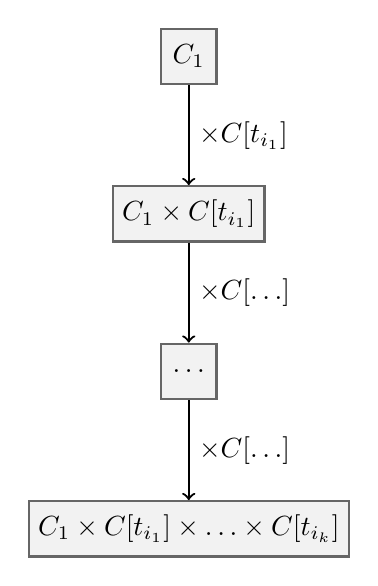
\begin{tikzpicture}[
		t/.style = {rectangle, draw=black!60, fill=black!5, thick, minimum size=20},
		r/.style = {->, thick}
		]
		
		%Nodes
		\node[t]	(1)	at	(0, 4)	{$C_1$};
		\node[t]	(2)	at	(0, 2)	{$C_1 \times C[t_{i_1}]$};
		\node[t]	(e)	at	(0, 0)	{$\ldots$};
		\node[t]	(i)	at	(0, -2)	{$C_1 \times C[t_{i_1}] \times \ldots \times C[t_{i_k}]$};
		
		%Lines
		\draw[r]	(1.south)	to	node[right]	{$\times C[t_{i_1}]$}	(2.north);
		\draw[r]	(2.south)	to	node[right]	{$\times C[\ldots]$}	(e.north);
		\draw[r]	(e.south)	to	node[right]	{$\times C[\ldots]$}	(i.north);
	\end{tikzpicture}
\end{minipage}
\hspace{10pt}
\begin{minipage}{0.1\textwidth}
	$$\equiv$$
\end{minipage}
\begin{minipage}{0.2\textwidth}
	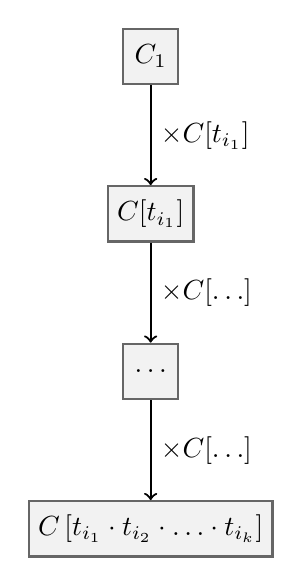
\begin{tikzpicture}[
		t/.style = {rectangle, draw=black!60, fill=black!5, thick, minimum size=20},
		r/.style = {->, thick}
		]
		
		%Nodes
		\node[t]	(1)	at	(0, 4)	{$C_1$};
		\node[t]	(2)	at	(0, 2)	{$C[t_{i_1}]$};
		\node[t]	(e)	at	(0, 0)	{$\ldots$};
		\node[t]	(i)	at	(0, -2)	{$C\left[ t_{i_1} \cdot t_{i_2} \cdot \ldots \cdot t_{i_k} \right]$};
		
		%Lines
		\draw[r]	(1.south)	to	node[right]	{$\times C[t_{i_1}]$}	(2.north);
		\draw[r]	(2.south)	to	node[right]	{$\times C[\ldots]$}	(e.north);
		\draw[r]	(e.south)	to	node[right]	{$\times C[\ldots]$}	(i.north);
	\end{tikzpicture}
\end{minipage}







\vspace{0.667in}

Тогда всё множество выходных конвейеров образует циклическую группу $C \left[ \prod_j t_{i_j} \right] \ = \ C \left[ \prod_i t_i^{a_i} \right]$. Если из них принудительно $b$ штук вернуть в начало -- то мы снова придём к теореме о делимости, и получим уменьшение периода группы: $C[s] \xrightarrow{-b} C[s-b]$






\vspace{0.5in}


\begin{minipage}{0.5\textwidth}
	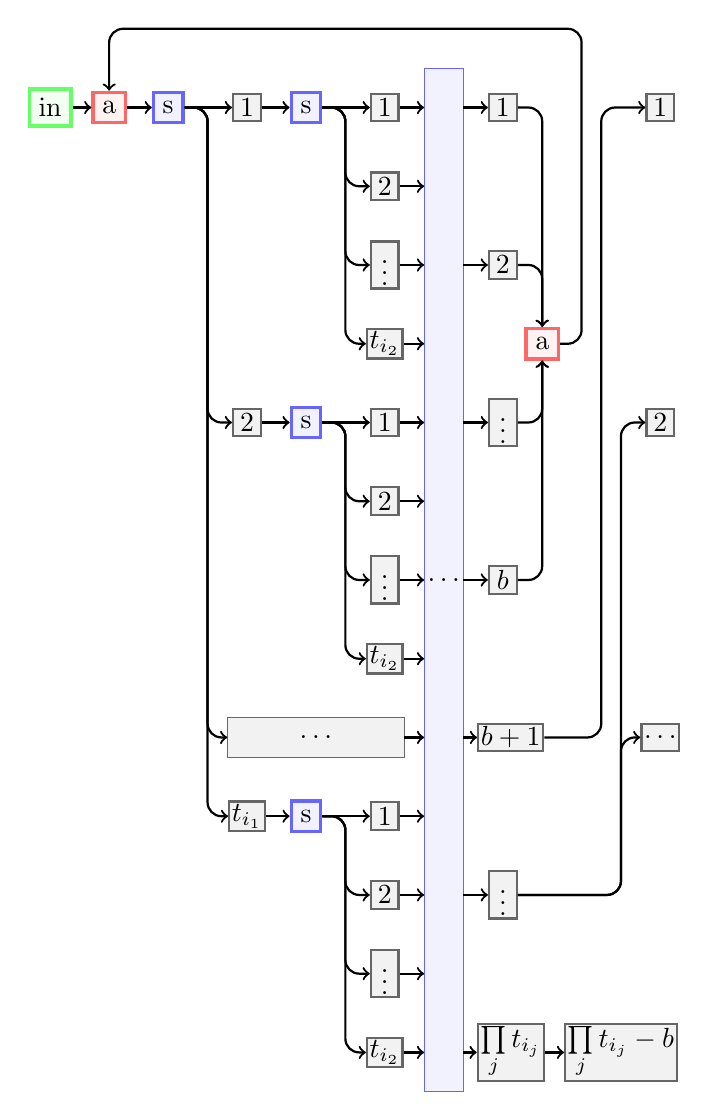
\begin{tikzpicture}[
		s/.style = {rectangle,	draw=blue!60,	fill=blue!5,	very thick, minimum size=10},
		a/.style = {rectangle,	draw=red!60,	fill=red!5,		very thick, minimum size=10},
		o/.style = {rectangle,	draw=green!60,	fill=green!5,	very thick, minimum size=10},
		t/.style = {rectangle,	draw=black!60,	fill=black!5,	thick, 		minimum size=10, inner sep=1pt},
		r/.style = {->, thick, rounded corners=5pt}
		]
		
		%Nodes
		\node[o]	(in)	at	(-3.25, 0)	{in};
		\node[a]	(a1)	at	(-2.5, 0)	{a};
		
		\node[s]	(s1)	at	(-1.75, 0)	{s};
		\node[t]	(t11)	at	(-0.75, 0)	{$1$};
		\node[t]	(t12)	at	(-0.75, -4)	{$2$};
		%\node[t]	(t1e)	at	(-1, -8)	{$\vdots$};
		\node[t]	(t1i)	at	(-0.75, -9)	{$t_{i_1}$};
		
		\node[s]	(s11)	at	(0, 0)		{s};
		\node[t]	(t121)	at	(1, 0)		{$1$};
		\node[t]	(t122)	at	(1, -1)		{$2$};
		\node[t]	(t12e)	at	(1, -2)		{$\vdots$};
		\node[t]	(t12i)	at	(1, -3)		{$t_{i_2}$};
		
		\node[s]	(s21)	at	(0, -4)		{s};
		\node[t]	(t221)	at	(1, -4)		{$1$};
		\node[t]	(t222)	at	(1, -5)		{$2$};
		\node[t]	(t22e)	at	(1, -6)		{$\vdots$};
		\node[t]	(t22i)	at	(1, -7)		{$t_{i_2}$};
		
		\node[s]	(si1)	at	(0, -9)		{s};
		\node[t]	(ti21)	at	(1, -9)		{$1$};
		\node[t]	(ti22)	at	(1, -10)	{$2$};
		\node[t]	(ti2e)	at	(1, -11)	{$\vdots$};
		\node[t]	(ti2i)	at	(1, -12)	{$t_{i_2}$};		
		
		% etc
		\draw[draw=blue!60,		fill=blue!5]	(1.5, 0.5)	rectangle node {$\ldots$} (2, -12.5);
		\draw[draw=black!60,	fill=black!5]	(-1, -7.75)	rectangle node {$\ldots$} (1.25, -8.25);
		
		\node[t]	(t1)	at	(2.5, 0)	{$1$};
		\node[t]	(t2)	at	(2.5, -2)	{$2$};
		\node[t]	(te1)	at	(2.5, -4)	{$\vdots$};
		\node[t]	(tb)	at	(2.5, -6)	{$b$};
		\node[t]	(tb+)	at	(2.6, -8)	{$b+1$};
		\node[t]	(te2)	at	(2.5, -10)	{$\vdots$};
		\node[t]	(tn)	at	(2.6, -12)	{$\prod\limits_{j} t_{i_j}$};
		
		\node[a]	(a2)	at	(3, -3)		{a};
		\node[t]	(t1`)	at	(4.5, 0)	{$1$};
		\node[t]	(t2`)	at	(4.5, -4)	{$2$};
		\node[t]	(te`)	at	(4.5, -8)	{$\ldots$};
		\node[t]	(tn`)	at	(4, -12)	{$\prod\limits_{j} t_{i_j} - b$};
	
		
		
		%Lines
		\draw[r]	(in.east)	to	(a1.west);
		\draw[r]	(a1.east)	to	(s1.west);
		
		\draw[r]	(s1.east)	to	(t11.west);
		\draw[r]	(s1.east)	to	(-1.25, 0)	|-	(t12.west);
		\draw[r]	(s1.east)	to	(-1.25, 0)	|-	(-1, -8);
		\draw[r]	(s1.east)	to	(-1.25, 0)	|-	(t1i.west);
		
		\draw[r]	(t11.east)	to	(s11.west);
		\draw[r]	(s11.east)	to	(t121.west);
		\draw[r]	(s11.east)	to	(0.5, 0)	|-	(t122.west);
		\draw[r]	(s11.east)	to	(0.5, 0)	|-	(t12e.west);
		\draw[r]	(s11.east)	to	(0.5, 0)	|-	(t12i.west);
		
		\draw[r]	(t12.east)	to	(s21.west);
		\draw[r]	(s21.east)	to	(t221.west);
		\draw[r]	(s21.east)	to	(0.5, -4)	|-	(t222.west);
		\draw[r]	(s21.east)	to	(0.5, -4)	|-	(t22e.west);
		\draw[r]	(s21.east)	to	(0.5, -4)	|-	(t22i.west);
		
		\draw[r]	(t1i.east)	to	(si1.west);
		\draw[r]	(si1.east)	to	(ti21.west);
		\draw[r]	(si1.east)	to	(0.5, -9)	|-	(ti22.west);
		\draw[r]	(si1.east)	to	(0.5, -9)	|-	(ti2e.west);
		\draw[r]	(si1.east)	to	(0.5, -9)	|-	(ti2i.west);
		
		\draw[r]	(t121.east)	to	(1.5, 0);
		\draw[r]	(t122.east)	to	(1.5, -1);
		\draw[r]	(t12e.east)	to	(1.5, -2);
		\draw[r]	(t12i.east)	to	(1.5, -3);
		\draw[r]	(t221.east)	to	(1.5, -4);
		\draw[r]	(t222.east)	to	(1.5, -5);
		\draw[r]	(t22e.east)	to	(1.5, -6);
		\draw[r]	(t22i.east)	to	(1.5, -7);
		\draw[r]	(1.25, -8)	to	(1.5, -8);
		\draw[r]	(ti21.east)	to	(1.5, -9);
		\draw[r]	(ti22.east)	to	(1.5, -10);
		\draw[r]	(ti2e.east)	to	(1.5, -11);
		\draw[r]	(ti2i.east)	to	(1.5, -12);
		
		\draw[r]	(2, 0)	to	(t1.west);
		\draw[r]	(2, -2)	to	(t2.west);
		\draw[r]	(2, -4)	to	(te1.west);
		\draw[r]	(2, -6)	to	(tb.west);
		\draw[r]	(2, -8)	to	(tb+.west);
		\draw[r]	(2, -10)	to	(te2.west);
		\draw[r]	(2, -12)	to	(tn.west);
		
		\draw[r]	(t1.east) 	-| 	(a2.north);
		\draw[r]	(t2.east) 	-| 	(a2.north);
		\draw[r]	(te1.east)	-| 	(a2.south);
		\draw[r]	(tb.east)	-| 	(a2.south);
		
		\draw[r]	(tb+.east)	to (3.75, -8) |- (t1`.west);
		\draw[r]	(te2.east)	to (4, -10) |- (t2`.west);
		\draw[r]	(te2.east)	to (4, -10) |- (te`.west);
		\draw[r]	(tn.east)	to	(tn`.west);
		
		\draw[r] 	(a2.east)	-| (3.5, 1) -| (a1.north);
	\end{tikzpicture}
\end{minipage}
\hspace{10pt}
\begin{minipage}{0.1\textwidth}
	$$\equiv$$
\end{minipage}
\begin{minipage}{0.2\textwidth}
	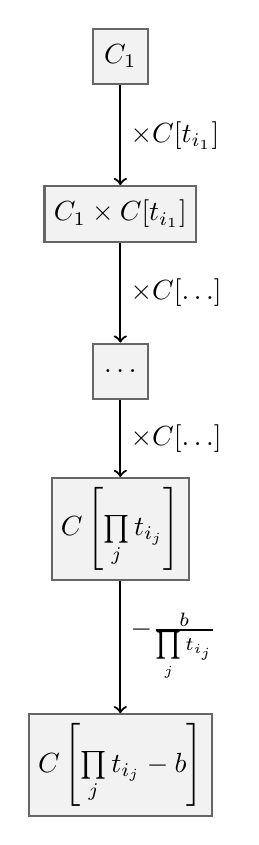
\begin{tikzpicture}[
		t/.style = {rectangle, draw=black!60, fill=black!5, thick, minimum size=20},
		r/.style = {->, thick}
		]
		
		%Nodes
		\node[t]	(1)	at	(0, 4)	{$C_1$};
		\node[t]	(2)	at	(0, 2)	{$C_1 \times C[t_{i_1}]$};
		\node[t]	(e)	at	(0, 0)	{$\ldots$};
		\node[t]	(n)	at	(0, -2)	{$C\left[ \prod\limits_{j} t_{i_j} \right]$};
		\node[t]	(*)	at	(0, -5)	{$C\left[ \prod\limits_{j} t_{i_j} - b\right]$};
		
		%Lines
		\draw[r]	(1.south)	to	node[right]	{$\times C[t_{i_1}]$}	(2.north);
		\draw[r]	(2.south)	to	node[right]	{$\times C[\ldots]$}	(e.north);
		\draw[r]	(e.south)	to	node[right]	{$\times C[\ldots]$}	(n.north);
		\draw[r]	(n.south)	to	node[right]	{$- \frac{b}{\prod\limits_{j} t_{i_j}}$}	(*.north);
	\end{tikzpicture}
\end{minipage}









\vspace{0.667in}

Схемы, приведённые справа являются биективными для любой неупрощённой диаграммы разделения, но как мы увидим далее, многие, первоначально кажущиеся сложными и громоздкими схемы -- можно довольно сильно сокращать, но тогда мы не сможем рисовать к ним данные схемы так просто. Тем более, такие схемы можно рисовать только для схем \textit{разделениея}, но не \textit{отделения}.









\vspace{0.5in}

\subsection{Теория графов}

Также хочется отметить, что, поскольку каждая схема является мультиорграфом -- то её можно описывать не в виде чертежа, а, например, в виде матрицы смежности:






%\vspace{0.5in}
\newpage

\begin{minipage}{0.25\textwidth}
	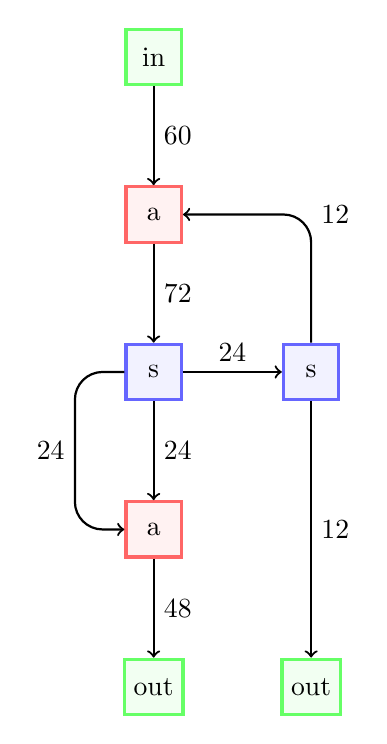
\begin{tikzpicture}[
		s/.style = {rectangle, draw=blue!60, fill=blue!5, very thick, minimum size=20},
		a/.style = {rectangle, draw=red!60, fill=red!5, very thick, minimum size=20},
		o/.style = {rectangle, draw=green!60, fill=green!5, very thick, minimum size=20},
		r/.style = {->, thick, rounded corners=10pt},
		]
		
		%Nodes
		\node[o]	(in)	at	(0, 4)	{in};
		\node[a]	(a1)	at	(0, 2)	{a};
		\node[s]	(s1)	at	(0, 0)	{s};
		\node[s]	(s2)	at	(2, 0)	{s};
		\node[a]	(a2)	at	(0, -2)	{a};
		\node[o]	(out1)	at	(0, -4)	{out};
		\node[o]	(out2)	at	(2, -4)	{out};
		
		%Lines
		\draw[r]	(in.south) 	to			node[right]	{$60$}	(a1.north);
		\draw[r]	(a1.south)	to			node[right]	{$72$}	(s1.north);
		\draw[r]	(s1.east)	to			node[above]	{$24$}	(s2.west);
		\draw[r]	(s2.north)	|-			node[right]	{$12$}	(a1.east);
		\draw[r]	(s1.west)	-| (-1, -1) node[left]	{$24$} |- (a2.west);
		\draw[r]	(s1.south)	to			node[right]	{$24$}	(a2.north);
		\draw[r]	(a2.south)	to			node[right]	{$48$}	(out1.north);
		\draw[r]	(s2.south)	to			node[right]	{$12$}	(out2.north);
	\end{tikzpicture}
\end{minipage}
\begin{minipage}{0.1\textwidth}
	$$\equiv$$
\end{minipage}
\begin{minipage}{0.4\textwidth}
	\begin{tabular}{|c|c|c|c|c|c|c|}
		\hline
		\textbackslash 
			&	a1&	a2&	s1&	s2&	out1&out2 \\
		\hline
		in&		1&	&	&	&	&	  \\
		\hline
		a1&		&	&	1&	&	&	  \\
		\hline
		a2&		&	&	&	&	1&	  \\
		\hline
		s1&		&	2&	&	1&	&	  \\
		\hline
		s2&		1&	&	&	&	&	1 \\
		\hline
		&&&&&& \\
		\hline
		in&		60&	&	&	&	&	  \\
		\hline
		a1&		&	&	72&	&	&	  \\
		\hline
		a2&		&	&	&	&	48&	  \\
		\hline
		s1&		&	24&	&	24&	&	  \\
		\hline
		s2&		12&	&	&	&	&	12\\
		\hline
	\end{tabular}
\end{minipage}




\vspace{0.5in}

Таблицу, удобства ради, давайте разделим на две части: сверху отметим обычную матрицу смежности для мультиорграфа: число в ячейке говорит о том, сколько рёбер идёт из одной вершины в другую. А снизу -- пропускную способность одного ребра.

\

Такой граф состоит из одной компоненты слабой связности, а все её компоненты сильной связности -- это области, благодоря которым происходит операция возврата. Посмотрев на полустепень исхода каждого из узлов компоненты сильной связности, можно выяснить, какой коэффициент усиления она реализует.

\

Однако матричный метод не является удобным, если все элементы $\mathbb{T}$ -- малы, а сам граф -- большой. Эффективность он преобретает, когда число выходных лент большое, а кратынх рёбер при этом мало.













\vspace{0.5in}

\subsection{Линейная алгебра}

Рассмотрим задачу перераспределения ресурсов между $n$ входами и $k$ выходами: схему перераспределения можно представить в виде матрицы:

$$
\left[
\begin{matrix}
	m_{11} & \ldots & m_{1n} \\
	\vdots & \ddots & \vdots \\
	m_{k1} & \ldots & m_{kn}
\end{matrix}
\right]
\times
\left[
\begin{matrix}
	\text{in}_1 \\
	\vdots \\
	\text{in}_n
\end{matrix}
\right]
=
\left[
\begin{matrix}
	\text{out}_1 \\
	\vdots \\
	\text{out}_k
\end{matrix}
\right]
$$

\

Рассмотрим матрицу $A \ := \ a_{ij} = \frac{\text{out}_i}{\text{in}_j}$. В ней можно выделить следующие классы значений:

%\

%Рассмотрим квадратную субматрицу $M' \subseteq M$. Если рассмотреть её диагональное решение -- то  ячейки $m_{ii}$ характеризуют, во сколько раз различаются стоящие друг напротив друга входы и выходы. Есть несколько принципиальных значений:

\begin{itemize}
	\item $a_{ij} = 1$ \\
		В этом случае конвейер надо просто провести прямо, без промежуточных преобразований
		
	\item $a_{ij} < 1$ \\
		В этом случае можно отделить соответствующую долю, а остаток станет новым входом, либо можно сохранить на следующие итерации.
	
	\item $a_{ij} > 1$ \\
		В таком случае итоговый конвейер получится, как сложение данного с некоторыми другими (или преобразованиями над ними)
\end{itemize}

\

%Когда мы находим ячейку со значением $1$ -- мы просто проводим прямой конвейер, и удаляем из матрицы соответствующие строку и столбец. Если мы решаем отделять стандартные и нестандартные дроби -- то удаляем только соответствующую строку матрицы. Как только в исходной субматрице удалены все доступные ячейки -- мы переходим к другим субматрицам. Такой процесс, очевидно, в какой-то момент закончится, и мы получим матрицу только со значениями $m_{ij} > 1$ -- тут следует искать уже полноценные решения. 

Если в такой матрице находится единичный элемент -- то в оригинальной матрице на этом же месте мы ставим $1$, а остальные значений в тех же столбце и строке -- заполняем нулями, а в первоначальной матрице они удаляются. Среди оставшихся элементов можно выбрать "диагональный" набор дольных значений, и по тем же принципам их занести в итоговую матрицу. Таким образом, должен остаться лишь набор элементов $a_{ij} > 1$. Тогда нам остаётся лишь честно искать решения.

\

Помочь в этом может следующая теорема: сумма значений в столбцах матрицы преобразования должна давать 1:



$$
\left[
\begin{matrix}
	m_{11} & \ldots & m_{1n} \\
	\vdots & \ddots & \vdots \\
	m_{k1} & \ldots & m_{kn}
\end{matrix}
\right]
\times
\left[
\begin{matrix}
	\text{in}_1 \\
	\vdots \\
	\text{in}_n
\end{matrix}
\right]
=
\left[
\begin{matrix}
	\text{out}_1 \\
	\vdots \\
	\text{out}_k
\end{matrix}
\right]
$$
$$
\sum_{i=1}^k m_{ji} = 1
$$


\

\noindent Таким образом, нам остаётся, всего-то навсего, решить систему $n+k$ уравнений и $nk$ переменных:

\begin{equation*}
	\begin{cases}
		m_{11}\cdot \text{in}_1 + \ldots + m_{1n}\cdot \text{in}_n = \text{out}_1 \\
		\vdots \\
		m_{k1}\cdot \text{in}_1 + \ldots + m_{kn}\cdot \text{in}_n = \text{out}_k \\
		m_{11} + \ldots + m_{k1} = 1 \\
		\vdots \\
		m_{1n} + \ldots + m_{kn} = 1 \\
	\end{cases}\,.
\end{equation*}

\

Как известно, такая система имеет единственное решение только если $nk = n+k$, что имеет только две пары целочисленных решений: $(0,0)$ и $(2,2)$. Если же точка находится где-то внутри -- то решение тривиально: соединение конвейеров, либо обычное отделение. В противном же случае -- решений бесконечно много. Если выходов больше, чем входов -- то входы можно банально поделить при помощи имеющихся у нас разделителей, и тогда, в какой-то момент мы сможем отделить все требуемые числа. Елси входов больше, чем выходов -- то наоборот, надо соединять.


























